
% ==========================================================

\chapter{Генерация и эволюция убегающих электронов в плазме токамаков и использование сцинтиляционных детекторов для их диагностики}
\label{ch:ch1}

В настоящей главе описаны различные механизмы генерации убегающих электронов в плазме токамака; затем будут рассказано о том, какие факторы влияют на движение убегающих электронов, приводя к уменьшению набираемой ими энергии. Затем будут рассмотрены различные механизмы диагностики убегающих электронов. В конце будет подробно рассмотрено устройство сцинтилляционных детекторов, с помощью которых возможно регистрировать тормозное излучение убегающих электронов. 

% ==========================================================

\section{Механизмы генерации убегающих электронов}
\label{sec:electronsGeneration}

В плазме токамаков имеют место несколько механизмов генерации убегающих электронов. Это:

\begin{itemize}
  \item <<традиционный>> механизм генерации убегающих электронов в электрическом поле;
  \item лавинный механизм, при котором первичные убегающие электроны при взаимодействии с электронами основной плазмы перевозят их в режим убегания;
  \item прочие механизмы, такие как генерация убегающих электронов при распаде трития или при комптоновском рассеянии гамма излучения.
\end{itemize}

Рассмотрим ниже эти механизмы подробнее.

% ----------------------------------------------------------

\subsection{Убегание электронов в сильных электрических полях в плазме}

Эффект убегания был предсказан в 1925 году \cite{Wilson1925} и развит в \cite{Dreicer1959}. Пусть в сильноионизованной плазме имеется электрическое поле $E$. Тогда для перехода в режим непрерывного ускорения сила, действующая на электрон со стороны электрического поля, должна превышать силу трения, вызванную кулоновскими столкновениями в плазме:

\begin{equation}
  \label{eq:runawayEq}
  e E >  m_e v_e \nu_{ei}(v_e)
\end{equation}
где $e$ и $m_e$ --- заряд и масса электрона, $\nu_{e}$ --- частота столкновений электрона, $v$ --- скорость электрона \cite{Wesson2004}. Частота кулоновских электрон-ионных столкновений зависит от скорости. Для случая, когда $v \gg \sqrt{ 2 T_e / m_e }$, где $T_e$ --- средняя температура электронов, частота электронных столкновений может быть представлена как 
\begin{equation*}
  \nu_{e}(v) = \frac{ 3 e^4 n \Lambda }{ 4 \pi \epsilon_0^2 m_e^2 v^3 }
\end{equation*} 
где $\Lambda$ --- кулоновский логарифм, $n$ --- концентрация плазмы \cite{Wesson2004}. Графики зависимости силы, действующей на электрон со стороны электрического поля, и силы трения, показаны на рисунке~\ref{fig:runawayForces}.

\begin{figure}[ht]
  \centerfloat{ 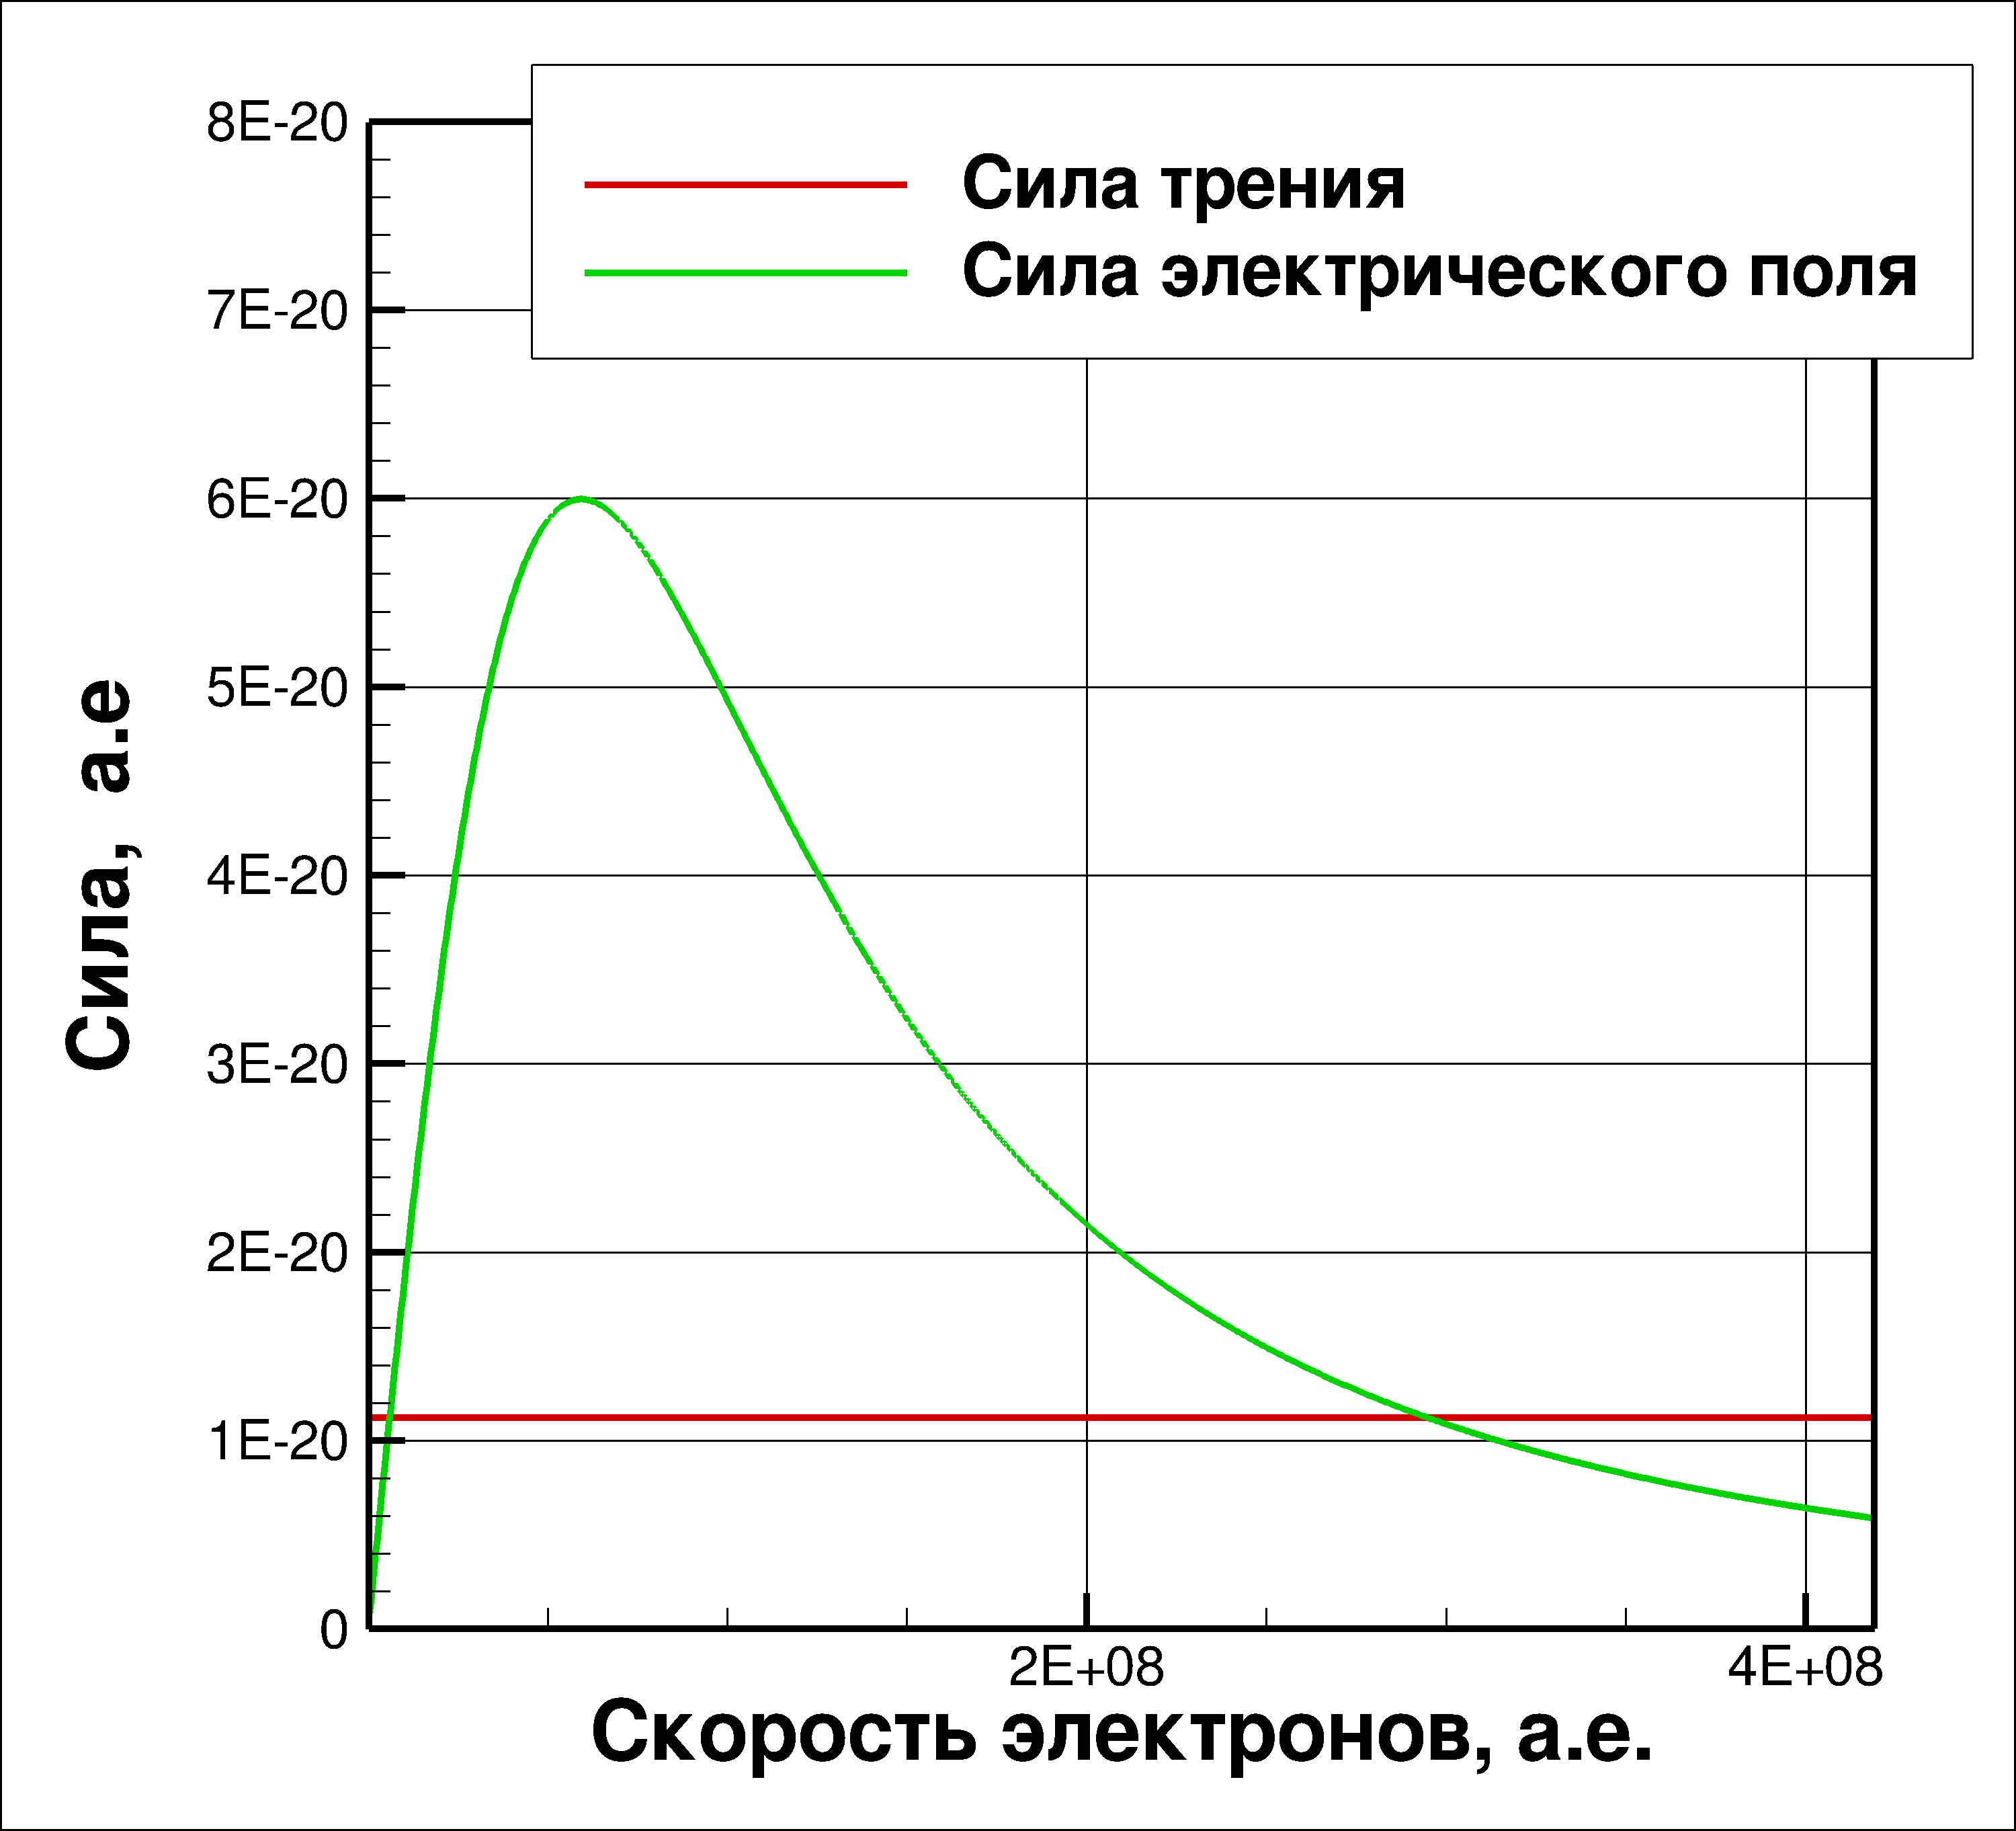
\includegraphics[width=0.60\linewidth]{runawayForces} }
  \caption{ Зависимотсть силы, действующей на электрон со стороны электрического поля и силы трения, которая вычислена по формуле $ C \cdot v/( v^2 + v_{Te}^2 )^{3/2} $~\cite{Golant1977}.}
  \label{fig:runawayForces}
\end{figure}

Можно заметить, что существует некая критическая скорость, начиная с которой неравенство \ref{eq:runawayEq} оказывается истинным. Эта критическая скорость равна
\begin{equation}
  \label{eq:critVelocity}
  v_c = \sqrt{ \frac{ 3 e^3 n \Lambda }{ 4 \pi \epsilon_0^2 m_e E } }
\end{equation}
Если каким-то образом образуется электрон со скоростью, больше критической скорости $v_c$, то он переходит в режим неограниченного ускорения. Такие электроны называются <<убегающими>> \cite{Golant1977}.

Можно рассчитать величину электрического поля, при котором в режим убегания переходят электроны с тепловой скоростью. Это поле оказывается равным 
\begin{equation}
  \label{eq:dreicerField}
  E_D = \frac{ n e^3 \Lambda }{ 4 \pi \epsilon_0^2 m_e v_{Te}^2 }
\end{equation}
и называется полем Дрейсера \cite{Dreicer1959,Golant1977,Wesson2004}. 

Когда электрическое поле достаточно мало, критическая скорость, рассчитанная по уравнению \ref{eq:critVelocity}, приближается к скорости света $c$. Для релятивистских электронов время замедления почти постоянно и существенного уменьшения силы трения с увеличением их энергии уже не происходит. Соответственно, для электрических полей, таких что
\begin{equation}
  \label{eq:criticalField}
  E < E_c = \frac{ n e^3 \Lambda }{ 4 \pi \epsilon_0^2 m_e c^2 }
\end{equation}
генерации убегающих электронов не происходит ни при каких обстоятельствах \cite{Wesson2004}.

На большем временном масштабе скорость убегания электронов определяется столкновительной диффузией в пространстве скоростей. По мере убегания более быстрых электронов они замещаются электронами, диффундирующими через хвост максвелловского распределения скоростей. Подробные расчеты дают следующую результирующую скорость убегания на единицу объема \cite{Wesson2004}: 
\begin{equation*}
  S_{re} = \frac{2}{ \sqrt{\pi} } n \nu_{e}(v_{Te}) \left( \frac{E}{E_D} \right)^{1/2} \exp\left( -\frac{E_D}{4 E} - \left( \frac{2 E_D }{E} \right)^{1/2} \right)
\end{equation*}


% ----------------------------------------------------------

\subsection{Лавинный эффект размножения убегающих электронов}

При кулоновских столкновениях между <<быстрыми>> убегающими электронами и <<медленными>> электронами основной плазмы первые могут передавать вторым часть своей энергией, переводя их в режим убегания \cite{Sokolov1979}. Очевидно, для работы этого процесса требуется, чтобы время жизни убегающего электрона было больше времени между кулоновскими столкновениями. Темп генерации оказывается пропорциональным числу уже существующих в плазме убегающих электронов \cite{Rozansky2012}.  Хотя на пробные частицы в плазме в основном влияют столкновения с большими прицельными параметрами и малым переданным импульсом, в этом процессе большее значение имеет меньшее число близких столкновений, передающих больший импульс. Соответствующие близкие столкновения в этом случае --- это те, которые поднимают медленный электрон выше критической скорости для убегания. 

Импульс, передаваемый медленному электрону быстрым электроном, в основном перпендикулярен скорости $v_f$ быстрого электрона и определяется выражением
\begin{equation*}
  m_e \Delta v \approx 2 m_e v_f \frac{r_0}{r}
\end{equation*}
где $r$ --- прицельный параметр, а $r_0 = e^2 / 4 \pi \epsilon_0 m_e v_f^2$ --- значение прицельного параметра для рассеяния на 90$^\circ$ \cite{Wesson2004}. 

Чтобы столкновение перенесло электрон в область убегания, $\Delta v$ должна быть больше критической скорости, определяемой уравнением \ref{eq:critVelocity}. С учётом этого требования, можно написать сечение для рождения убегающего электрона:
\begin{equation*}
  \sigma(v_f) = \frac{ e E }{ 3 n m_e v_f^2 \Lambda }
\end{equation*}
Считая убегающие электроны релятивистскими, можно положить что $v_f = c$. Тогда скорость рождения новых убегающих электронов оказывается равна следующей величине \cite{Rozansky2012}:
\begin{equation}
  \label{eq:avalanch}
  \frac{ d n_r }{ d t } = n_r \nu_e(c) \left( \frac{E}{E_c} - 1 \right) / \left( 2 \Lambda \right)
\end{equation}
Множитель $E/E_c - 1 $ в формуле \ref{eq:avalanch} показывает, что лавинный механизм генерации убегающих электронов имеет пороговый характер.

Подробно теория генерации убегающих электронов изложена в \cite{Rosenbluth1997}. Лавинный механизм генерации убегающих электронов неоднократно наблюдался в экспериментах; впервые оно было экспериментально обнаружено на токамаке TEXTOR, вероятно имеет место во время срывов на токамаках TFTR, Tore Supra, JT-60U и JET \cite{Gill2002,Helander2002}, было зарегистрировано на токамаке TCABR \cite{Galvao2001}. Анализ распределения по энергии убегающих электронов позволяет предположить, что лавинный механизм может быть доминирующим при генерации убегающих электронов во время срывов, а в срывах JET кажется трудным объяснить ток, переносимый убегающими электронами, не прибегая к этому механизму \cite{Helander2002}.


% ----------------------------------------------------------

\subsection{Прочие механизмы генерации убегающих электронов}

Прочие механизмы генерации убегающих электронов носят скорее экзотический характер и не являются существенными на современных установках, однако могут оказывать влияние на более крупных токамаках будущего. Эти механизмы могут служить источником первичных убегающих электронов, которые могут потом размножаться по лавинному механизму за счёт кулоновских столкновений.

При радиоактивном распаде трития, который будет являться одним из компонентов топливной смеси промышленных термоядерных установок, образуется электрон \cite{Burrows1990}:
\begin{equation*}
  T \rightarrow {}^3_2 He + e^{-} + \bar{ \nu_e }
\end{equation*}
Период полураспада трития составляет $ \tau_T = 4500 $ дней, максимальная энергия рождённых в ходе распада электронов равна $ E_{max} = 18.6$~кэВ \cite{MartinSolis2017}. Число убегающих электронов, рождённых за счёт подобного механизма, составляет

\begin{equation*}
  \left( \frac{ d n_{re} }{ d t } \right) \approx \ln(2) \frac{ n_T }{ \tau_T } F_{\beta}(\varepsilon_c)
\end{equation*}
где $\varepsilon_c = m_e v_c^2 / 2$, а 
\begin{equation*}
  F_{\beta}(\varepsilon_c) = \int\limits_{\varepsilon_c}^{ \varepsilon_{max} } f_{\beta}(\varepsilon) d\varepsilon 
\end{equation*}

Тут $ f_{\beta}(\varepsilon) $ --- функция распределения рождаемых в ходе распада электронов от энергии, нормированная на единицу \cite{MartinSolis2017}. Очевидно, что если скорость рождённых в ходе распада электронов меньше, чем скорость, необходимая для перехода в режим убегания, то данный механизм генерации убегающих электронов не функционирует.

В токамаке ИТЭР происходит активация стенок за счёт нейтронов, рождённых в ходе термоядерной DT реакции. Это приводит к тому, что конструкции токамака начинают генерировать гамма излучение. Гамма кванты могут рассеиваться на электронах плазмы, передавая им свою энергию и тем самым потенциально переводя их в режим убегания. Количество создаваемых таким механизмом электронов оказывается равным 
\begin{equation*}
  \left( \frac{ d n_{re} }{ d t } \right) \approx n_e \int \Gamma_{\gamma}(E_{\gamma}) \sigma(E_{\gamma}) d E_{\gamma} 
\end{equation*}
где $\Gamma_{\gamma}(E_{\gamma})$ --- поток гамма квантов с энергией $E_{\gamma}$, $\sigma(E_{\gamma})$ --- сечение рассеяния \cite{MartinSolis2017}.

Графики зависимости скорости генерации убегающих электронов от величины $\varepsilon_c$ для обоих описанных механизмов показан на рисунке~\ref{fig:solisGeneration}.

\begin{figure}[ht]
    \begin{minipage}[b][][b]{0.49\linewidth}\centering
        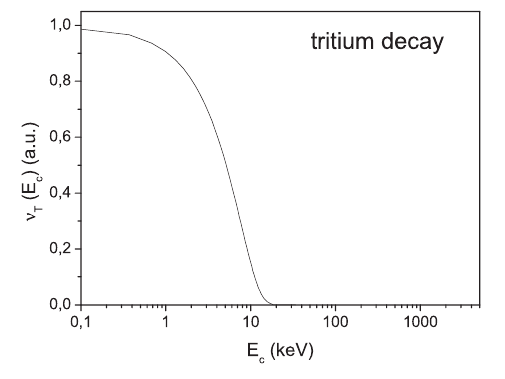
\includegraphics[width=0.95\linewidth]{solisRunawayRenerationTritium} \\ а)
    \end{minipage}
    \hfill
    \begin{minipage}[b][][b]{0.49\linewidth}\centering
        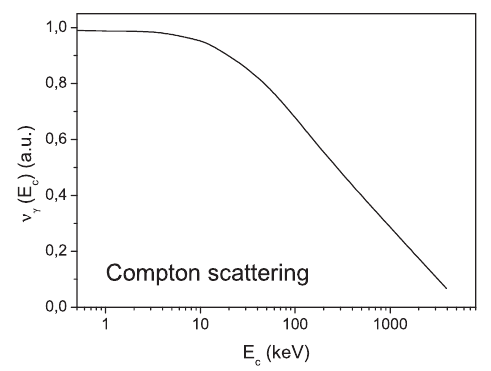
\includegraphics[width=0.95\linewidth]{solisRunawayRenerationCompton} \\ б)
    \end{minipage}
    \caption{ Зависимость скорости генерации убегающих электронов для механизма генерации из электронов, рождённых в ходе радиоактивного распада трития (а) и для механизма генерации за счёт комптоновского рассеяния (б). По вертикальной оси отложена величина $\nu \equiv (1/n_e) \cdot ( dn_r / dt ) $, нормированная на 1 при $\varepsilon_c = 0$; по горизонтальной --- критическая энергия, равная $v_c^2 m_e / 2 $ \cite{MartinSolis2017}. }
    \label{fig:solisGeneration}
\end{figure}


% ==========================================================

\section{Механизмы ограничения энергии убегающих электронов}

На реальных установках существует ряд механизмов, которые ограничивают максимальную энергию убегающих электронов: 

\begin{itemize}
  \item ограничение энергии, набираемой электроном в электрическом поле токамака за время своего ускорения;
  \item синхротронное и тормозное излучение;
  \item дрейфовое смещение орбиты;
  \item взаимодействие с возмущением магнитного поля;
  \item плазменные неустойчивости.
\end{itemize}

Рассмотрим эти механизмы подробнее.

% ----------------------------------------------------------

\subsection{Ограничение энергии, набираемой электроном в электрическом поле токамака}

Ускорение убегающего электрона в плазме можно описать с помощью следующих уравнений в первом приближении \cite{MartinSolis1998,Bakhtiari2005}:
\begin{equation}
  \label{eq:AccelerationRunaways}
  \begin{alignedat}{1}
    \frac{ d p_{\parallel} }{ d t } & = e E_{\parallel} - \frac{ n_c e^4 \Lambda m_e }{ 4 \pi \epsilon_0^2 } \gamma ( Z_{eff} + 1 + \gamma ) \frac{ p_{\parallel} }{ p^3 } - ( F_s + F_b ) \frac{ p_{\parallel} }{ p }   \\
    \frac{ d p }{ d t } & = e E_{\parallel} \frac{ p_{\parallel} }{ p } - \frac{ n_c e^4 \Lambda m_e }{ 4 \pi \epsilon_0^2 } \frac{ \gamma^2 }{ p^2 } - ( F_s + F_b )
  \end{alignedat}  
\end{equation}
где $ p_{\parallel} $ --- компонента импульса, параллельная магнитному (тороидальному) полю, $p$ --- полный импульс убегающего электрона, $\gamma = 1 + p^2 / ( m_e c )^2$ --- релятивистский гамма-фактор, $Z_{eff}$ --- эффективный заряд ионов в плазме. 

Первый член правой части уравнений~\ref{eq:AccelerationRunaways} отвечает за за ускорение электронов в тороидальном электрическом поле, второй --- за торможение в результате столкновений с частицами в плазме. Последнее слагаемое, включающее в себя сумму сил $F_s + F_b$, отвечает за радиационные потери энергии за счёт синхротронного и тормозного излучения и будет рассмотрен позднее.

Если в нулевом приближении пренебречь торможением электрона и радиационными потерями, то должно быть очевидно, что за время разряда токамака с момента своего рождения электрон может набрать только конечную энергию, которая определяется временем ускорения и электрическим полем в плазме за время ускорения. Эта величина может быть грубо оценена в предположении, что $v = c$ как

\begin{equation}
  \label{eq:MaxRunawayEnergyLimit}
  \varepsilon(t) = \frac{ e c }{ 2 \pi R_0 } \int \limits_{t_b}^{t} V_{loop}(t') d t'
\end{equation}
где $t_b$ --- время перехода электрона в режим убегания, $V_{loop}$ --- напряжение обхода. Очевидно, что реальная энергия электрона всегда будет меньше этой величины \cite{Shevelev2019th}.

% ----------------------------------------------------------

\subsection{Синхротронное и тормозное излучение}

В уравнениях~\ref{eq:AccelerationRunaways} присутствует сила, отвечающая за торможение убегающих электронов в результате потерь энергии на синхротронное излучение, которая равна \cite{MartinSolis1998, MartinSolis1999} 
\begin{equation*}
  F_s = \frac{2}{3} r_e m_e c^2 \left( \frac{v}{c} \right)^3 \gamma^4 \langle \frac{1}{R^2} \rangle
\end{equation*}
где $r_e = e^2/(4 \pi \epsilon_0 m_e c^2 )$ --- классический радиус электрона, $v$ --- скорость электрона, $R$ --- радиус кривизны траектории убегающего электрона. Орбита электрона в токамаке 
состоит из двух частей: движения ведущего центра вдоль силовых линий магнитного поля и ларморовского вращения. В приближении, что большой радиус токамака $R_0$ намного больше, чем ларморовский радиус $r_g$, можно написать выражение для среднего радиуса кривизны траектории убегающего электрона \cite{MartinSolis1998}:
\begin{equation*}
  \langle \frac{1}{R^2} \rangle \approx \frac{1}{R_0^2} + \frac{ \sin(\theta)^4 }{r_g^2}
\end{equation*}
где $\theta$ --- пинч-угол. 

На рис.~\ref{fig:solisRunawayPhaseDiagram} показана фазовая диаграмма решения системы уравнений~\ref{eq:AccelerationRunaways}. Для каждого значения электрического поля существуют два значения $p_{\parallel}$ и $p_{\perp}$, соответствующие двум особым точкам $P_1$ и $P_2$. Эти две особые точки имеют вполне определенный физический смысл: ветвь седловой точки $P_1$ дает критическую энергию для генерации убегающих электронов, а устойчивый фокус в точке $P_2$ даёт энергетический предел для генерируемых убегающих электронов.

\begin{figure}[ht]
  \centerfloat{ 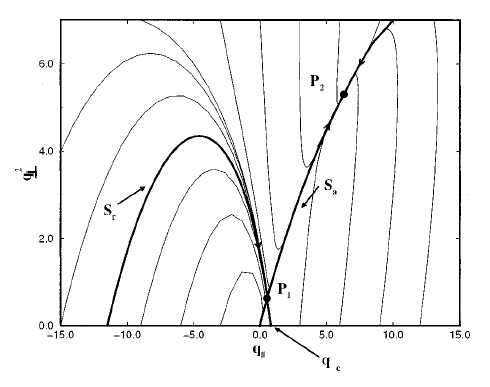
\includegraphics[width=0.60\linewidth]{solisRunawayPhaseDiagram} }
  \caption{ Фазовая диаграмма решения системы уравнений~\ref{eq:AccelerationRunaways} в координатах $q_{\parallel} = p_{\parallel}/(m_e c)$ и $q_{\perp} = p_{\perp}/(m_e c)$ для параметров ( $E_{\parallel} m_e c^2 )/(T_e E_D ) = 4.4$, $ 1 + Z_{eff} = 4 $, $ 2 \epsilon_0 B_0^2 / 3 n_e = 0.65 $, $ ( m_e c / e B_0 R_0 )^2 \cdot 2 \epsilon_0 B_0^2 / 3 n_e = 2.3 \cdot 10^{-8} $, $F_b = 0$ ~\cite{MartinSolis1998}.}
  \label{fig:solisRunawayPhaseDiagram}
\end{figure}

Предельными траекториями частиц, проходящих через точки $P_1$ и $P_2$, являются сепаратрисы $S_r$ и $S_a$. Сепаратриса $S_r$ делит фазовое пространство на две области, причем область вне $S_r$ составляет область убегания: все электроны, первоначально находившиеся вне $S_r$, в конце концов будут двигаться вдоль $S_a$ к устойчивому фокусу $P_2$. Электроны, изначально находившиеся внутри $S_r$, будут двигаться в начало координат, т.е. они не переходят в режим убегания. Устойчивая точка $P_2$ является следствием учёта радиационных потерь в уравнениях. Убегающие электроны не непрерывно ускоряются тороидальным электрическим полем, вместо этого они достигают максимальной энергии, когда мощность, излучаемая электроном, равна получению энергии от электрического поля.  

Сила, действующая на убегающий электрон вследствие потерь энергии на тормозное излучение, может быть записана для однокомпонентной плазмы как \cite{Bakhtiari2005}
\begin{equation*}
  F_b = \frac{4}{137} n_e ( Z_{eff} + 1 ) m_e c^2 \gamma r_e^2 \left( \ln 2 \gamma - \frac{1}{3} \right)
\end{equation*}

Отметим, что синхротронное излучение зависит от тороидального магнитного поля, большого радиуса токамака и скорости электронов, а сила, действующая на электрон из-за тормозного излучения, не зависит от магнитного поля и большого радиуса, но зависит от концентрации и эффективного заряда $Z_{eff}$ в плазме. При нормальной работе термоядерного токамака $Z_{eff}$ имеет низкое значение, чуть выше единицы, но в случае чрезвычайной ситуации, когда токамак необходимо быстро отключить, может быть введено огромное количество примесей с высоким $Z$, повышая тем самым $Z_{eff}$. 

% ----------------------------------------------------------

\subsection{Дрейфовое смещение орбиты}

С ростом энергии электрона траектория убегающего электрона будет смещаться в сторону слабого магнитного поля токамака. В некоторый момент траектория электрона пересекается с лимиттером или с первой стенкой токамака, в результате чего электрон гибнет \cite{MartinSolis1999,Carbajal2017}. В предположении плоского профиля тока по плазме это происходит при энергии \cite{Knoepfel1979,MartinSolis1999}

\begin{equation*}
  \gamma = \left[ \left( 2 R_0 ( 1 - r_c / r_l ) \frac{I_p}{17000} \right)^2 + 1 \right]^{\frac{1}{2}}
\end{equation*}
где $r_c$ --- малый радиус, на котором электрон перешёл в режим убегания, $r_l$ --- радиус, на котором расположен лимиттер или первая стенка, $I_p$ --- ток по плазме. Пример расчётных орбит показан на рис.~\ref{fig:breizmanOrbits}

\begin{figure}[ht]
  \centerfloat{ 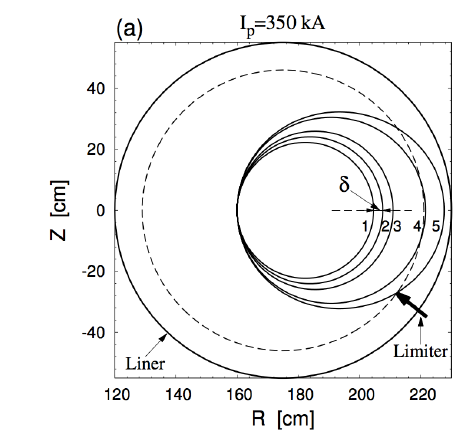
\includegraphics[width=0.60\linewidth]{breizmanOrbits} }
  \caption{ Траектории ведущих центров убегающих электронов при различных значениях энергии. Токамак TEXTOR, $I_p = 350$~кА, $B_0 = 2.5$~Т, кривые 1--5 соответствуют энергиям 10~кэВ, 10~МэВ, 20~МэВ, 40~МэВ, 46~МэВ\cite{Breizman2019,Abdullaev2016}.}
  \label{fig:breizmanOrbits}
\end{figure}

% ----------------------------------------------------------

\subsection{Взаимодействие с возмущениями магнитного поля}

Магнитное поле токамака является неоднородным из-за конечного числа обмоток. Резонанс между движением электронов по ларморовской окружности и гармониками пульсации тороидального поля, возникающими вследствие конечного числа обмоток, увеличивает компоненту скорости, перпендикулярную направлению магнитного полю \cite{MartinSolis1998,MartinSolis1999,Laurent1990}. Взаимодействие с n-й гармоникой пульсаций тороидального поля происходит при энергии электрона 
\begin{equation*}
  \gamma_n \approx \frac{ e B_0 R_0 }{ n N_c m_e c }
\end{equation*}
где $N_c$ --- число катушек тороидального поля, $n$ --- номер тороидальной гармоники. Эффективность механизма пульсаций для ограничения энергии убегающих электронов сильно зависит от амплитуды пульсаций: при заданном электрическом поле для эффективного взаимодействия необходима достаточно большая амплитуда пульсаций. В токамаке сила пульсаций больше для низких номеров тороидальных гармоник и быстро затухает по радиусу от края плазмы. Поэтому следует ожидать, что эффекты будет наиболее существенным в периферийных областях плазмы \cite{MartinSolis1998}.

% ----------------------------------------------------------

\subsection{Плазменные неустойчивости}

На существование убегающих электронов в плазме так же оказывают влияние различные неустойчивости. 

Стоит особо отметить веерную неустойчивость. Как правило, эта неустойчивость развивается в разрядах с невысокой плотностью (менее $10^{19}$~м${}^{-3}$. Неустойчивость проявляется в виде коротких (10--100~мкс) периодических всплесков увеличения диамагнетизма плазмы; время между соседними всплесками намного превышает продолжительность каждого из них (1--2~мс).  Одновременно с измене- изменением диамагнетизма наблюдается резкое увеличение интенсивности рентгеновского и синхротронного излучения плазмы, меняется напряжение на обходе плазменного шнура. Развитие этой неустойчивости может ограничивать энергию убегающих электронов и приводить к аномальной диффузии к стенке токамака. \cite{Parail1978,Leontovich1982}

Существенно влияние различных МГД неустойчивостей, которые приводят к выходу убегающих электронов, существующих в плазме, на переферию плазмы, а электроны с периферии выходят на стенки или лимиттер токамака. Соответствующие всплески рентгеновского излучения неоднократно наблюдались на небольших установках \cite{Shevelev2016,Shevelev2018}. 

% ==========================================================

\section{Методы диагностики убегающих электронов}

Диапазон энергий убегающих электронов очень широк: это значения от тепловых энергий электронов (несколько кэВ во время типичного разряда) до десятков МэВ. Этот широкий диапазон энергий не может быть исследован какой-либо одной диагностикой~\cite{Breizman2019}. Поэтому для диагностики энергии убегающих электронов, питч-угла и пространственного распределения используются различные методы диагностики, которые кратко будут рассмотрены ниже.

% ----------------------------------------------------------

\subsection{Тормозное излучение}

Тормозное излучение является одним из наиболее широко используемых диагностических инструментов для диагностики убегающих электртонов в токамаках~\cite{Breizman2019,Cooper2016,Shevelev2013,Chugunov2011}. Строго говоря, термин  <<тормозное излучение>> относится к любому излучению, обусловленному замедлением заряженных частиц, но мы будем использовать здесь тормозное излучение в более узком смысле — излучение электронов, замедляющихся в веществе. Тормозное излучение от убегающих электронов может быть объемным тормозным излучением тонкой мишени, когда убегающие электроны рассеиваются ионами плазмы, или тормозным излучением толстой мишени, когда убегающие электроны попадают на компоненты, обращенные к плазме. Объемная эмиссия преобладает, когда убегающие электроны хорошо удерживаются, тогда как поверхностное тормозное излучение преобладает во время быстрой потери электронов, например связанная с выбросами в ходе МГД нействойчивости или в ходе выхода на лимиттер.~\cite{Breizman2019}

Энергетический спектр испускаемых квантов жёсткого рентгеновского излучения имеет верхнюю границу при энергии падающего электрона и пик примерно при 1/4~энергии падающего электрона~\cite{Seltzer1985,Kuznetsov1974,Shevelev2013}. Угловое распределение квантов тормозного излучения имеет тенденцию к изотропии до 1~МэВ (мягкий и средний диапазоны рентгеновского излучения); при больших энергиях излучение приобретает анизотропный характер и преимущественно направлено в ту же сторону, куда двигается электрон. Электрон-ионные столкновения преобладают над электрон-электронными столкновениями при образовании тормозного излучения, и, таким образом, тормозное излучение имеет зависимость от заряда ядра как $Z^2$, что делает излучение весьма чувствительным к содержанию примесей в плазме~\cite{Seltzer1985,Breizman2019}.

Обнаружение фотонов тормозного излучения обычно осуществляется с использованием полупроводниковых детекторов при более низких энергиях и сцинтилляционных детекторов при более высоких энергиях. В диапазоне 1--10~кэВ в токамаках наиболее распространены Si детекторы, а в диапазоне 10--1000~кэВ чаще используются детекторы CdTe из-за их более высокой тормозной способности~\cite{Esposito2003}. Полупроводниковые детекторы непосредственно обнаруживают ток от электронно-дырочных пар, создаваемых фотонами, и могут достигать очень высокой эффективности обнаружения фотонов (в некоторых случаях вплоть до единичной квантовой эффективности). В сцинтилляционных детекторах используются прозрачные материалы высокой плотности для обнаружения излучения видимого света, возникающего в результате погложения кванта жёсткого рентгена. Излучение видимого света обусловлено рекомбинацией электронов в связанные состояния, тогда как механизмами поглощения энергии налетающих квантов являются фотоэлектрический эффект (для квантов с энергией менее 1~МэВ), комптоновское рассеяние при промежуточных энергиях и образование электронно-позитронных пар при высокорелятивистских энергиях (>10 МэВ). Сцинтилляционные материалы, используемые в токамаках, включают в себя такие материалы как NaI(Tl)~\cite{Shevelev2004,Vlainic2015}, BGO~\cite{Shevelev2013,James2011} и LaBr3(Ce)~\cite{Shevelev2016,Nocente2010}; разные сцинтилляторы отличаются такими параметрами, как уровень сигнала, скорость затухания сигнала, возможность раздеоения сигналов от нейтронов и рентгена, а так же ценой. Подсчет сигналов от фотонов тормозного излучения может производиться либо в токовом режиме, либо в режиме спектроскопии. В токовом режиме просто измеряется полный фототок от детектора (обычно пропорциональный потоку энергии фотонов)~\cite{Savrukhin2002}. В режиме спектроскопии измеряются амплитуды отдельных импульсов квантов, что позволяет реконструировать функцию распределения фотонов по энергии.~\cite{Shevelev2013,Khilkevitch2013} Таким образом, режим спектроскопии предоставляет больше информации, но является более сложным в экспериментальном плане, требуя более высокого коэффициента усиления, лучшей защиты от шума и лучшей коллимации. Экранирование (блокировка от рассеянного излучения) и коллимация (сужение поля зрения до определенной хорды обзора) в целом представляют собой проблему при измерении тормозного излучения убегающих электронов, поскольку часть жёсткого рентгеновского спектра чрезвычайно трудно заблокировать, для этого требуется несколько сантиметров свинцового экрана для значительного ослабления.~\cite{Cooper2016,Breizman2019}

% ----------------------------------------------------------

\subsection{Синхротронное излучение}

Обычно с точки зрения принятной в диагностики высокотемпературной плазмы терминологии, под <<синхротронным излученим>> понимают излучение света релятивистскими электронами в магнитном поле, а <<циклотронным излчением>> называют излучение нерелятивистскими электронами в магнитном поле; это не вполне соответствует приятым обозначениям в других областях науки~\cite{Breizman2019}. В токамаках среднего и большого размера гироскопическое движение электронов обычно является основной причиной генерации излучения. В этом случае мощность синхротронного излучения сильно зависит от кинетической энергии электронов (как $\gamma^4$) и от их питч-угла (как $\theta^2$)~\cite{Pankratov1999}. Сам питч-угол зависит от содержания примесей в плазме, что приводит к синхротронному излучению, которое имеет тенденцию сильно увеличиваться с увеличением количества примесей. Для типичных наблюдаемых почти равновесных функций распределения энергии убегающих электронов после срывов в токамаках среднего размера синхротронное излучение исходит преимущественно от убегающих электронов в диапазоне энергий 30--40 МэВ с пиками в среднем инфракрасном диапазоне (2--4 мкм)~\cite{Stahl2013}. Излучение имеет очень сильную анизотропию по направлению движения пучка, поэтому для его регистрации требуется система с тангенциальным обзором.~\cite{Breizman2019} 

% ----------------------------------------------------------

\subsection{Циклотронное излучение}

Измерение электронной циклотронной эмиссии (ЭЦЭ) в микроволновом (ghbvthyj 50--200~ГГц) диапазоне частот --- одна из первых диагностик токамаков~\cite{Costley1974}. В нем используются либо быстрые системы (радиометры), либо медленные системы (интерферометры). Быстрая диагностика электрон-циклотронной эмиссии обычно использует гетеродинные радиометры для разделения микроволнового сигнала на отдельные каналы, каждый из которых имеет отдельный полосовой фильтр для выделения определенной полосы частот, что дает очень быстрые (более 1~МГц) измерения излучения ЭЦЭ с грубым (около 1~ГГц) спектральным разрешением. Более медленные (менее 100~Гц), широкополосные и с более высоким спектральным разрешением (менее 1~ГГц) измерения ЭЦЭ обычно получают с помощью интерферометров Майкельсона. Измерения ЭЦЭ обычно проводятся при одной поляризации, либо перпендикулярной тороидальному магнитному полю, либо параллельной магнитному полю. Направление наблюдения обычно радиально внутрь токамака, с тем чтобы измерить профиль радиальной температуры плазмы.~\cite{Breizman2019}

Быстрые электроны приводят к росту уровня сигнала ЭЦЭ и вызывают уширение функции распределения, что делает ЭЦЭ потенциально полезной диагностикой для анализа убегающих электронов. На сегодняшний день, однако, сложность интерпретации вклада ЭЦЭ от убегающих электронов ограничивает использование этой диагностики в основном качественным использованием.~\cite{Breizman2019} 

% ----------------------------------------------------------

\subsection{ Инфракрасное излучение }

Использование для диагностики инфракрасного излучения может использоваться для изучения структуры тепловых нагрузок, возникающих в результате выхода убегающих электронов на стенку токамака, на протяженных участках внутренней поверхности камеры. Хотя по анализу инфракрасного излучения можно определить поток энергии, передаваемый от убегающих электронов конструкциям камеры, но на практике это оказывается довольно сложной задачей. Инфракрасная диагностика используется на токамаках JET и DIII-D~\cite{Breizman2019,Lehnen2009,Hollmann2017}.

% ----------------------------------------------------------

\subsection{Прочие методы диагностики}

В принципе, эмиссия примесных линий так же может быть использована для диагностики убегающих электронов, но в этой области сделано мало исследований. Ряд измерений проводились на DIII-D, так же проводились измерения K$\alpha$ излучения криптона с энергией 12.6~кэВ после газонапуска.~\cite{Breizman2019}

На токамаке TEXTOR использовалась зондовая диагностика в области периферийной SOL плазмы. Наконечник зонда содержал десять кристаллов YSO (Y2SiO3:Ce), соединенных оптическими волокнами с фотоумножителями. Сцинтилляторы были защищены вольфрамовой защитой. Энергетический диапазон этой диагностики составлял примерно 5–20 МэВ.~\cite{Kudyakov2008} 

Так же можно использовать и черенковские зонды, которые так же содержат экранированный прозрачный материал вместе и оптоволокно для вывода сигнала на фотодетектор. В качестве материалов для таких зондов используется алмаз и AlN. Черенковское излучение возникает в любом материале при попадании частиц со сверхсветовой скоростью, например энергии электронов это энергии выше 58~кэВ в алмазе или 175~кэВ в пластике. Черенковские детекторы использовались на нескольких токамаках, например Tore Supra и COMPASS~\cite{Zebrowski2018}.

При нормальном сценарии работы токамака в эмиссии нейтронов токамака обычно преобладают реакции синтеза D-D, особенно в экспериментах с нагревом пучка. Однако при наличии достаточно больших популяций убегающих электронов или при использовании плазмы H или He образование нейтронов может быть в первую очередь связано с фотоядерными ядерными реакциями в материале стенки. Это нейтронное излучение может быть зарегистрировано многими нейтронными детекторами. Обычно фотонейтронный сигнал может быть использован только в качестве детектора выхода высокоэнергетичных электронов на стенку без возможности определения энергетических характеристик электронов.~\cite{Breizman2019,Strachan1977}

Томсоновское рассеяние лазерного света на электронах является хорошо известной диагностикой токамака, и способность томсоновского рассеяния видеть немаксвелловские (но нерелятивистские) электроны была отмечена на токамаке C-MOD. Релятивистский аналог, индуцированное лазером обратное комптоновское рассеяние, был предложен для диагностики убегающих электронов, но пока не реализован.~\cite{Breizman2019,Pieroni1975,Wurden2014}

% ==========================================================

\section{Использование сцинтилляционных детекторов для регистрации тормозного излучения от убегающих электронов}

В настоящей работе в основном будет рассматриваться диагностика убегающих электронов по тормозному излучению с помощью сцинтиляционных детекторов. Ниже будет более подробно освещено устройство и особенности таких детекторов.

% ----------------------------------------------------------

\subsection{ Взаимодействие гамма излучения с веществом}

Когда гамма-квант проходит через детектор, он может взаимодействовать с материалом детектора в основном посредством одного из следующих процессов \cite{Grozdanov2021,Knoll2010}: 
\begin{itemize}
  \item фотоэлектрический эффект;
  \item комптоновское рассеяние;
  \item образование электрон-позитронных пар.  
\end{itemize}
Все эти процессы приводят к частичному или полному переходу энергии гамма-квантов в энергию электронов. В ходе взаимодействия с веществом квант либо полностью исчезает, либо рассеивается под значительным углом.~\cite{Knoll2010}

В процессе фотоэлектрического поглощения квант взаимодействует с атомом поглотителя, при котором этот квант полностью исчезает. Вместо него энергичный фотоэлектрон выбрасывается атомом из одной из его связанных оболочек. Взаимодействие происходит с атомом в целом и не может происходить со свободными электронами. Для гамма-лучей достаточной энергии наиболее вероятным источником фотоэлектрона является наиболее прочно связанная или К-оболочка атома. Фотоэлектрон появляется с энергией, определяемой выражением
\begin{equation*}
  E_e = h \nu - E_b
\end{equation*}
где $E_b$ --- энергия связи фотоэлектрона в его исходной оболочке. При энергиях гамма-излучения более нескольких сот кэВ фотоэлектрон уносит большую часть первоначальной энергии фотона. 

Помимо фотоэлектрона, взаимодействие создает также ионизированный атом-поглотитель с вакансией в одной из его связанных оболочек. Эта вакансия быстро заполняется за счет захвата свободного электрона из среды и/или перераспределения электронов с других оболочек атома. Следовательно, также могут генерироваться один или несколько характеристических рентгеновских фотонов. Хотя в большинстве случаев эти рентгеновские лучи повторно поглощаются близко к исходному участку сцинтиллятора за счет фотоэлектрического поглощения с участием менее прочно связанных оболочек, их миграция и возможное ускользание от детекторов излучения могут влиять на функцию отклика детектора. В некоторых случаях испускание оже-электрона может происходить вместо характеристического рентгеновского излучения при переносе энергии возбуждения атома.~\cite{Knoll2010}

Процесс взаимодействия комптоновского рассеяния происходит между падающим квантом гамма-излучения и электроном в поглощающем материале. Чаще всего это преобладающий механизм взаимодействия для энергий гамма-излучения, типичных для радиоизотопных источников. При комптоновском рассеянии входящий квант гамма-излучения отклоняется на угол $\theta$ по отношению к его первоначальному направлению. Квант передает часть своей энергии электрону (предполагается, что изначально он находится в состоянии покоя), который называется электроном отдачи. Поскольку возможны все углы рассеяния, энергия, передаваемая электрону, может варьироваться от нуля до значительной доли энергии гамма-излучения. Выражение, связывающее передачу энергии и угол рассеяния для любого заданного взаимодействия, можно просто получить, написав одновременные уравнения сохранения энергии и импульса. Используя символы, определенные на схеме из рисунка~\ref{fig:electronComptonScattering}, можно показать, что
\begin{equation*}
  h \nu' = \frac{ h \nu }{ 1 + \frac{h \nu }{ m_e c^2  } ( 1 - \cos(\theta) ) }
\end{equation*}

\begin{figure}[ht]
  \centerfloat{ 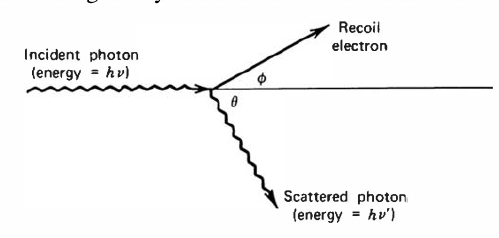
\includegraphics[width=0.60\linewidth]{electronComptonScattering} }
  \caption{ Схема комптоновского рассеяния.~\cite{Knoll2010}.}
  \label{fig:electronComptonScattering}
\end{figure}

При малых углах рассеяния $\theta$ при рассеянии электрону передается очень мало энергии. Часть первоначальной энергии всегда сохраняется в налетающем кванте, даже при предельном значении $\theta = \phi$. Вероятность комптоновского рассеяния на атоме поглотителя зависит от числа электронов, доступных в качестве рассеивающих мишеней, и, следовательно, линейно возрастает с его зарядом $Z$.~\cite{Knoll2010}

Если энергия кванта излучения превышает удвоенную энергию массы покоя электрона (1,02~МэВ), то становится возможным процесс образования электрон-позитронных пар. При энергиях гамма-излучения, превышающих этот порог всего на несколько сотен кэВ, вероятность образования пар невелика. Однако этот механизм взаимодействия становится преобладающим при увеличении энергии в области многих МэВ. При взаимодействии (которое должно происходить в кулоновском поле ядра) гамма-квант исчезает и заменяется электронно-позитронной парой. Вся избыточная энергия, переносимая фотоном выше 1,02~МэВ, необходимой для создания пары, переходит в кинетическую энергию, разделяемую позитроном и электроном. Поскольку позитрон впоследствии аннигилирует после замедления в поглощающей среде, два аннигиляционных фотона обычно образуются как вторичные продукты взаимодействия. Последующая судьба этого аннигиляционного излучения оказывает важное влияние на реакцию детекторов гамма-излучения.~\cite{Knoll2010}

Не существует простого выражения для вероятности образования пары на ядро, но ее величина изменяется примерно пропорционально квадрату атомного номера вещества поглотителя. Важность образования пар резко возрастает с ростом энергии.~\cite{Knoll2010}

Относительная важность трех процессов, описанных выше, для различных поглотителей и энергий гамма-излучения проиллюстрирована на рисунке~\ref{fig:gammaProcessesImpotance}. Линия слева представляет энергию, при которой фотоэлектрическое поглощение и комптоновское рассеяние равновероятны в зависимости от атомного номера поглотителя. Линия справа представляет энергию, при которой комптоновское рассеяние и рождение пар равновероятны. Таким образом, на графике определяются три области, в которых преобладают фотоэлектрическое поглощение, комптоновское рассеяние и образование пар.~\cite{Knoll2010}

\begin{figure}[ht]
  \centerfloat{ 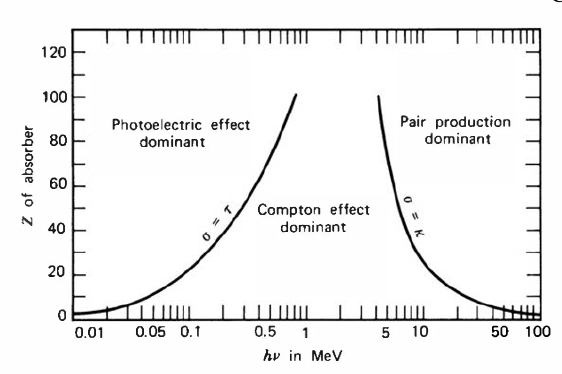
\includegraphics[width=0.60\linewidth]{gammaProcessesImpotance} }
  \caption{ Относительная важность трех основных типов взаимодействия гамма-излучения с веществом. Линии показывают значения $Z$ и $h \nu$, при которых вклад двух соседних эффектов эквивалентен.~\cite{Evans1955}.}
  \label{fig:gammaProcessesImpotance}
\end{figure}

Помимо комптоновского рассеяния может иметь место другой тип рассеяния, при котором квант гамма-излучения когерентно взаимодействует со всеми электронами атома-поглотителя. Этот процесс когерентного рассеяния или рэлеевского рассеяния не возбуждает и не ионизирует атом, а квант гамма-излучения сохраняет свою первоначальную энергию после рассеяния. Поскольку энергия практически не передается, этим процессом обычно пренебрегают в основных обсуждениях взаимодействий гамма-излучения.~\cite{Knoll2010}

% ----------------------------------------------------------

\subsection{ Сцинтилляторы }

Регистрация ионизирующего излучения с помощью света, выделяемого при сцинтилляции некоторыми материалами, является одним из старейших методов регистрации. Процесс сцинтилляции остается одним из наиболее полезных методов обнаружения и спектроскопии широкого спектра излучений. Идеальный сцинтилляционный материал должен обладать следующими свойствами~\cite{Knoll2010}:
\begin{itemize}
  \item Он должен преобразовывать кинетическую энергию заряженных частиц в регистрируемый свет с высокой эффективностью сцинтилляции;
  \item Это преобразование должно быть линейным --- светоотдача должна быть пропорциональна выделенной энергии в как можно более широком диапазоне;
  \item Среда должна быть прозрачной для длины волны собственного излучения для хорошего сбора света;
  \item Время затухания индуцированной люминесценции должно быть коротким, чтобы можно было генерировать быстрые импульсы сигнала;
  \item Материал должен быть хорошего оптического качества и производиться в достаточно больших размерах, чтобы представлять интерес в качестве практического детектора;
  \item Его показатель преломления должен быть близок к показателю преломления стекла ($\approx$~1,5), чтобы обеспечить эффективную передачу сцинтилляционного света на фотоумножитель или другой датчик света.
\end{itemize}

Ни один материал одновременно не отвечает всем этим критериям, и выбор конкретного сцинтиллятора всегда является компромиссом между этими и другими факторами. Наиболее широко применяемые сцинтилляторы включают неорганические кристаллы галогенидов щелочных металлов, из которых предпочтительным является йодид натрия, а также жидкости и пластмассы на органической основе. Неорганические вещества, как правило, имеют лучший световой поток и линейность, но, за некоторыми исключениями, имеют относительно медленное время отклика. Органические сцинтилляторы обычно быстрее, но дают меньше света. Предполагаемое применение также оказывает большое влияние на выбор сцинтиллятора. Высокое значение $Z$ компонентов и высокая плотность неорганических кристаллов благоприятствуют их выбору для гамма-спектроскопии, тогда как органические вещества часто предпочтительнее для бета-спектроскопии и обнаружения быстрых нейтронов (из-за содержания в них водорода).~\cite{Knoll2010}

Процесс флуоресценции --- это мгновенное испускание видимого излучения веществом после его возбуждения каким-либо образом. Принято выделять несколько других процессов, которые также могут приводить к излучению видимого света. Фосфоресценция соответствует излучению света с большей длиной волны, чем флуоресценция, и с характерным временем, которое обычно намного меньше. Замедленная флуоресценция приводит к тому же спектру излучения, что и быстрая флуоресценция, но опять же характеризуется гораздо более длительным временем излучения после возбуждения. Чтобы быть хорошим сцинтиллятором с точки зрения использования в детекторах, материал должен преобразовывать как можно большую долю энергии падающего излучения в мгновенную флуоресценцию, сводя при этом к минимуму обычно нежелательные вклады в фосфоресценцию и замедленную флуоресценцию. При работе сцинтилляторов в импульсном режиме свет, который может вносить вклад в выходной импульс, обычно ограничивается мгновенной флуоресценцией, потому что время формирования импульса измерительной схемы установлено намного меньшим, чем обычное время затухания фосфоресценции и задержанной флуоресценции. Затем этот долгоживущий свет распределяется более или менее случайным образом во времени между сигнальными импульсами и достигает датчика света в виде отдельных фотонов, которые часто невозможно отличить от случайного шума. Напротив, сцинтилляторы, которые работают в токовом режиме при постоянном освещении, будут генерировать установившийся ток сигнала, который пропорционален общему световому выходу, и все компоненты затухания будут вносить вклад, пропорциональный их абсолютной интенсивности. По этой причине световыход, измеренный от сцинтиллятора, работающего в импульсном режиме, может оказаться ниже, чем полученный от стационарного тока, зарегистрированного от того же сцинтиллятора. Сцинтилляционные детекторы токового режима режима, работающие в условиях быстрого изменения интенсивности излучения, будут страдать от эффектов памяти или ``послесвечения'', если долгоживущие компоненты спада значительны.~\cite{Knoll2010}

В таблице~\ref{tab:scintiilatorProperties} представленны характеристики некоторых часто используемых сцинтилляторов, используемых при диагностике плазмы. Атомная структура сцинтилляторов LaBr3(Ce) и NaI(Tl) показана на рисунке~\ref{fig:scintillatorAtomicStructure}.

\begin{table} [htbp]
    \centering
    \begin{threeparttable}
      \caption{ Параметры некоторых неорганических сцинтилляторов.~\cite{Grozdanov2021} }
        \label{tab:scintiilatorProperties}
        \begin{tabular}{| p{7cm} | p{2cm} | p{2cm} | p{2cm} | }
            \hline
            Хараектристика   & BGO & NaI(Tl) & LaBr3(Ce) \\
            \hline
            Световыход, фотон/кэВ & 9 & 38 & 63 \\
            Время спада импульса, нс & 300 & 250 & 16 \\
            Длина волны излучения (максимум), нм & 480 & 415 & 380 \\
            Показатель преломления на этой дине волны & 2.15 & 1.85 & $\approx$1.9 \\
            Плотность, г/см${}^3$ & 7.13 & 3.68 & 5.08 \\
            Длина, на которой полгощается 50\% илучения 662~кэВ, см & 1.0 & 2.5 & 1.8 \\
            \hline
        \end{tabular}
    \end{threeparttable}
\end{table}

\begin{figure}[ht]
  \centerfloat{ 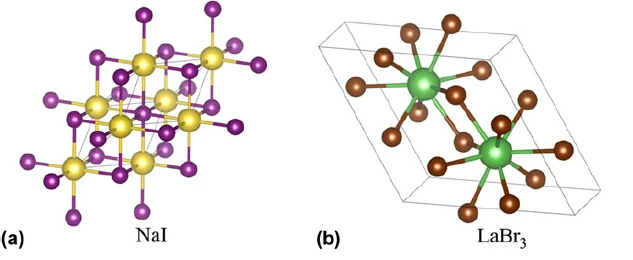
\includegraphics[width=0.80\linewidth]{scintillatorAtomicStructure} }
  \caption{ Атомная структура элементарных ячеек кристаллов NaI~(a) и LaBr3(Ce)~(b).~\cite{Schleife2016}.}
  \label{fig:scintillatorAtomicStructure}
\end{figure}


%В детекторе сцинтилляционный кристалл обычно оптически соединяется с ФЭУ, сигнал с которого дальше передаётся на АЦП. При соединении могут использоваться различные приёмы, позволяющие увелчиить количество собираемого света, например использоваться фоконы. 

% ----------------------------------------------------------

\subsection{Конструкция детектора}

Широкое использование сцинтилляционного счета в детектировании излучений и спектроскопии было бы невозможно без наличия устройств для преобразования крайне слабого светового выхода сцинтилляционного импульса в соответствующий электрический сигнал. Фотоумножитель (ФЭУ) замечательно справляется с этой задачей, преобразовывая световые сигналы, которые обычно состоят не более чем из нескольких сотен фотонов, в полезный импульс тока, не добавляя к сигналу большого количества случайного шума. Фотодиоды так же могут использоваться для этой цели, но происходит это обычно гораздо реже.~\cite{Knoll2010}

Схема типичного сцинтилляционного детектора представлена на рисунке~\ref{fig:scintillatorSchemeExample}.

\begin{figure}[ht]
  \centerfloat{ 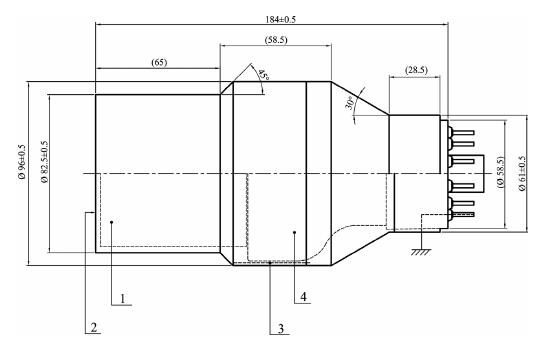
\includegraphics[width=0.80\linewidth]{scintillatorSchemeExample} }
  \caption{ Схема сцинтилляционного детектора из работы~\cite{Grozdanov2021}. Цифрами на рисунке обозначены: 1 --- кристалл LaBr3(Ce), 2 --- алюминиевый корпус, 3 --- магнитный экранирован, 4 --- ФЭУ Hamamatsu R10233. Габаритные размеры указаны в миллиметрах.}
  \label{fig:scintillatorSchemeExample}
\end{figure}


% ----------------------------------------------------------

\subsection{Функция отклика детектора}

Процесс взаимодействия гамма-кванта с веществом является случайным процессом, и невозможно предсказать, какая часть его начальной энергии будет поглощена детектором для данного единичного события. Однако можно определить вероятность обнаружения определенной доли начальной энергии гамма-кванта путем измерения распределения энергии регистрируемых импульсов для большого числа событий от моноэнергетического источника. Это распределение называется функцией отклика.~\cite{Grozdanov2021} 

Обычно в гамма-спектроскопии высокого разрешения при анализе сложных спектров интерес представляют только полные пики поглощения всей энергии, так как их положения пропорциональны начальным энергиям соответствующих гамма-квантов. Иногда одиночные и двойные пики убегания также считаются полезными частями спектра. Остальная часть спектра в основном образует континуум, который служит нежелательным фоном для н пиков от низкоэнергетичных квантов. Основная цель анализа такого спектра состоит в том, чтобы как можно точнее определить положение пика полного поглощения энергии и число событий в нём, при этом непрерывный фон обычно аппроксимируется гладкой функцией и вычитается. С другой стороны, знание функции отклика детектора позволяет использовать не только события из пиков полного поглощения или выхода энергии, но и из непрерывной части спектра, либо суммируя эти события с событиями полного энергетического пика. пиков поглощения, используя процедуру деконволюции или принимая во внимание знание формы континуума в процедуре фиттнга.~\cite{Grozdanov2021}

На рисунке~\ref{fig:scintillatorResponseExample} представлены функции отклика детекторов на основе различных материалов. 

\begin{figure}[ht]
  \centerfloat{ 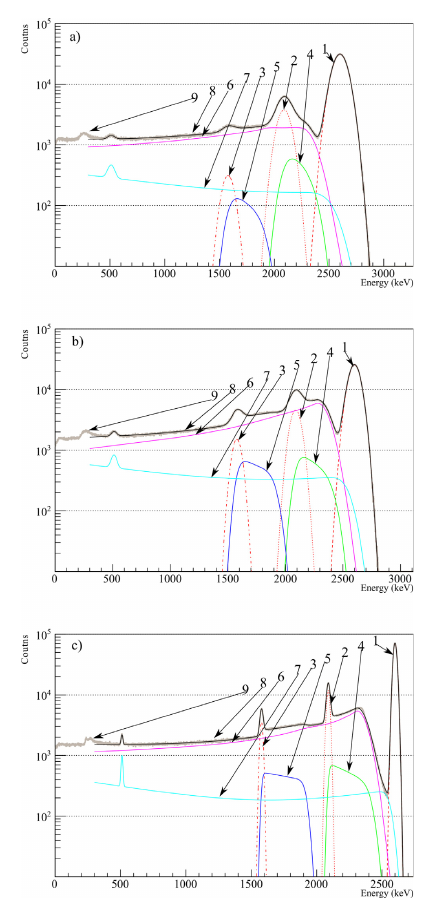
\includegraphics[width=0.50\linewidth]{scintillatorResponseExample} }
  \caption{ Фиттированные функции отклика детекторов BGO~(a), NaI(Tl)~(b) и LaBr3(Ce)~(c) на $\gamma$-кванты с энергией 2,6~МэВ. Обозначены компоненты функций отклика: 1 --- пик полного поглощения энергии, 2 --- пик одиночного вылета, 3 --- пик двойного вылета, 4 --- комптновоский край с одиночным вылетом, 5 — комптоновский край с двойным вылетом, 6 --- вклад внутреннего рассеяния, 7 --- вклад внешнего рассеяния, 8 --- функция полного отклика и 9 --- результаты моделирования.~\cite{Grozdanov2021}}
  \label{fig:scintillatorResponseExample}
\end{figure}

% ==========================================================

\FloatBarrier
\section{Выводы к главе 1}

В настоящей главе рассмотрены механизмы возникновения убегающих электронов: прежде всего, это ускорение электронов в электрическом поле с переходом в режим убегания, затем --- лавинный эффект, при котором кулоновские столкновения первичных убегающих электронов приводят с обычными электронами плазмы приводят к переходу последних в режим убегания, а так же ряд прочих механизмов (радиоактивный распад трития, рассеяние гамма излучения на свободных электронах). Рассмотрены механизмы, ограничивающие энергию убегающих электронов: ограничение из-за конечного времени жизни электрона, синхротронное и тормозное излучение, дрейфовое смещение орбиты, взаимодействие с возмущениями магнитного поля, плазменные неустойчивости.

Затем были рассмотрены методы диагностики убегающих электронов: по тормозному и синхротронному излучению, циклотронному излучению, инфракрасному излучению. Были рассмотрены принципы работы сцинтилляционных детекторов излучения, с помощью которых возможно регистрировать жёсткое рентгеновское излучение, генерируемое убегающими электронами.

% ----------------------------------------------------------

\FloatBarrier
